% !TeX program = lualatex
\documentclass[a4paper]{article}
\usepackage{amsmath}
\usepackage[utf8]{inputenc}
\usepackage{amsmath}
\usepackage{cancel}
\usepackage[portuguese]{babel}
\usepackage{fancybox}
\usepackage{amssymb}
\usepackage{capt-of}
\usepackage{pgfplots}
\usepackage{tikz}
\usepackage{polynom}
\usepackage{adjustbox}
\usepackage{pgfplots}
\usepackage{graphics}
\usepgfplotslibrary{fillbetween}
\usetikzlibrary{matrix}
\usetikzlibrary{calc}
\usetikzlibrary{patterns}
\usetikzlibrary{decorations.pathreplacing}

\tikzset{
	CE/.style={column #1/.style={nodes={text width=43mm}}}
}
%\tikzset{
	%	CA/.style={column #1/.style={nodes={text width=15mm}}}
	%}

\begin{document}
	\section*{Exercício 1}\textbf{Para cada uma das alíneas seguintes, indique:}
\begin{center}
\adjustbox{valign=t}{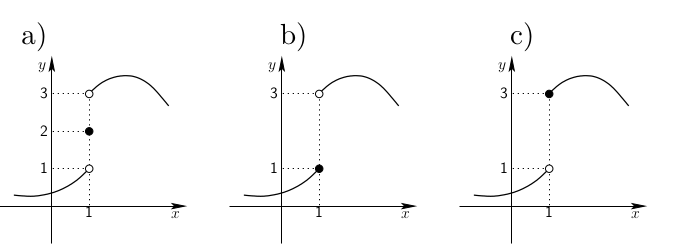
\includegraphics[width=1.3\textwidth]{images/ex1ficha13p1.png}}
\end{center}
\begin{center}
\adjustbox{valign=t}{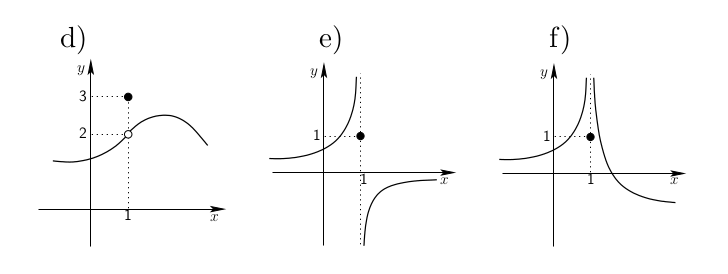
\includegraphics[width=1.3\textwidth]{images/ex1ficha13p2.png}}
\end{center}
\begin{itemize}
	\item[i)]\textbf{$\lim\limits_{x \to 1^-}f(x)$;}
	\begin{itemize}
		\item[a)]\text{$1$;}
		\item[b)]\text{$1$;}
		\item[c)]\text{$1$;}
		\item[d)]\text{$2$;}
		\item[e)]\text{$+\infty$;}
		\item[f)]\text{$+\infty$;}
	\end{itemize}
	\item[ii)]\textbf{$\lim\limits_{x \to 1^+}f(x)$;}
		\begin{itemize}
		\item[a)]\text{$3$;}
		\item[b)]\text{$3$;}
		\item[c)]\text{$3$;}
		\item[d)]\text{$2$;}
		\item[e)]\text{$-\infty$;}
		\item[f)]\text{$+\infty$;}
	\end{itemize}
	\item[iii)]\textbf{$f(1)$.}
		\begin{itemize}
		\item[a)]\text{$2$;}
		\item[b)]\text{$1$;}
		\item[c)]\text{$3$;}
		\item[d)]\text{$3$;}
		\item[e)]\text{$1$;}
		\item[f)]\text{$1$;}
	\end{itemize}
\end{itemize}
\section*{Exercício 2}\textbf{Sendo a função $\it{h}$ definida, em $\mathbb{R}$,por}
\[h(x)=\begin{cases}
	\text{$2x$,se $x \geq 3$}\\ 
	\text{$x^2-3$ se $x < 3$}
\end{cases}\]
\textbf{Calcule}

\textbf{$\lim\limits_{x \to 5} \it{h(x)}$;}

\[\lim\limits_{x \to 5} h(x)=\lim\limits_{x \to 5} 2x = 10\]

\textbf{$\lim\limits_{x \to -\infty} \it{h(x)}$;}

\[\lim\limits_{x \to -\infty} h(x)=\lim\limits_{x \to -\infty} x^2-3= +\infty\]	

\textbf{$\lim\limits_{x \to 3^{-}} \it{h(x)}$;}

\[\lim\limits_{x \to 3^{-}} h(x)=\lim\limits_{x \to 3^{-}} x^2-3 = 6\]

\textbf{$\lim\limits_{x \to 3^{+}} \it{h(x)}$;}

\[\lim\limits_{x \to 3^{+}} h(x)=\lim\limits_{x \to 3^{+}} 2x = 6\]
\textbf{Diga se existe $\lim\limits_{x \to 3} h(x)$.}

\text{Existe limite pois só existe um limite.}

\section*{Exercício 3}\textbf{Calcule, se existirem, os seguintes limites:}
	
\subsection*{a)}\textbf{$\lim\limits_{x \to 3^{-}}\ \frac{x^2}{x-3}$}
	\[\lim\limits_{x \to 3^{-}}\ \frac{x^2}{x-3}=\frac{9}{0^{-}}=-\infty\] 
	
\subsection*{b)}\textbf{$\lim\limits_{x \to -1^{+}}\ \frac{4x-3}{x+1}$}
\[\lim\limits_{x \to -1^{+}}\ \frac{4x-3}{x+1}=\frac{-7}{0^{+}}=-\infty\] 

\subsection*{c)}\textbf{$\lim\limits_{x \to 0^{+}}\ \left(\frac{1}{x}-\frac{1}{x^2}\right)$}
\[\lim\limits_{x \to 0^{+}}\ \left(\frac{1}{x}-\frac{1}{x^2}\right)=\lim\limits_{x \to 0^{+}}\ \frac{x-1}{x^2}=\frac{-1}{0^{+}}=-\infty\] 

\subsection*{d)}\textbf{$\lim\limits_{x \to 0}\ \frac{5x^3+8x^2}{3x^4-16x^2}$}
\[\lim\limits_{x \to 0}\ \frac{5x^3+8x^2}{3x^4-16x^2}=\lim\limits_{x \to 0}\ \frac{\cancel{x^2}\left(5x+8\right)}{\cancel{x^2}\left(3x^2-16\right)}=-\frac{1}{2}\]

\subsection*{e)}\textbf{$\lim\limits_{x \to 2}\ \frac{x^3-5x^2+8x-4}{x^3-3x^2+4}$}

\text{C.A.}

\textbf{$x^3-5x^2+8x-4$}
\\

\polyhornerscheme[x=2]{x^3-5x^2+8x-4}


\polyhornerscheme[x=2]{x^2-3x+2}

\textbf{$x^3-5x^2+8x-4=(x-2)^2\left(x-1\right)$}\\


\textbf{$x^3-3x^2+4=(x-2)^2\left(x+1\right)$}\\



\polyhornerscheme[x=2]{x^3-3x^2+4}

\polyhornerscheme[x=2]{x^2-x-2}


\[\lim\limits_{x \to 2}\ \frac{\cancel{(x-2)^2}\left(x-1\right)}{\cancel{(x-2)^2}\left(x+1\right)}=\frac{1}{3}\]

\subsection*{f)}\textbf{$\lim\limits_{x \to -\infty}\ \frac{2x^2+5x}{3x+2-4x^2}$}

\[\lim\limits_{x \to -\infty}\ \frac{2x^2+5x}{3x+2-4x^2}=\lim\limits_{x \to -\infty}\ \frac{\cancel{x^2}\left(2+\cancelto{0}{\frac{5}{x}}\right)}{\cancel{x^2}\left(\cancelto{0}{\frac{3}{x}}+\cancelto{0}{\frac{2}{x^2}}-4\right)}=-\frac{1}{2}\]

\subsection*{g)}\textbf{$\lim\limits_{x \to +\infty}\ \frac{x^2}{x^3+9}$}

\[\lim\limits_{x \to +\infty}\ \frac{x^2}{x^3+9}=\lim\limits_{x \to +\infty}\ \frac{\cancel{x^2}}{\cancel{x^2}\left(x+\cancelto{0}{\frac{9}{x^2}}\right)}=\frac{1}{+\infty}=0\]

\subsection*{h)}\textbf{$\lim\limits_{x \to +\infty}\ \left(\sqrt{x^2+1}-\sqrt{x^2-1}\right)$}

\[\lim\limits_{x \to +\infty}\ \left(\sqrt{x^2+1}-\sqrt{x^2-1}\right)=\lim\limits_{x \to +\infty}\ \frac{\cancel{x^2}}{\cancel{x^2}\left(x+\cancelto{0}{\frac{9}{x^2}}\right)}=\frac{1}{+\infty}=0\]

\subsection*{i)}\textbf{$\lim\limits_{x \to -\infty}\ e^{-2x}$}
\[\lim\limits_{x \to -\infty}\ e^{-2x}=e^{+\infty}=+\infty\]

\subsection*{j)}\textbf{$\lim\limits_{x \to -\infty}\ \frac{2^x}{3^x}$}
\[\lim\limits_{x \to -\infty}\ \frac{2^x}{3^x}=\lim\limits_{x \to -\infty}\ \left(\frac{2}{3}\right)^x=\left(\frac{2}{3}\right)^{-\infty}=+\infty\]
\end{document}
